\documentclass[tikz,border=4pt]{standalone}
\usepackage{ctex}
\usepackage{amsmath}
\usepackage{pgfplots}
\pgfplotsset{compat=1.18}
\begin{document}
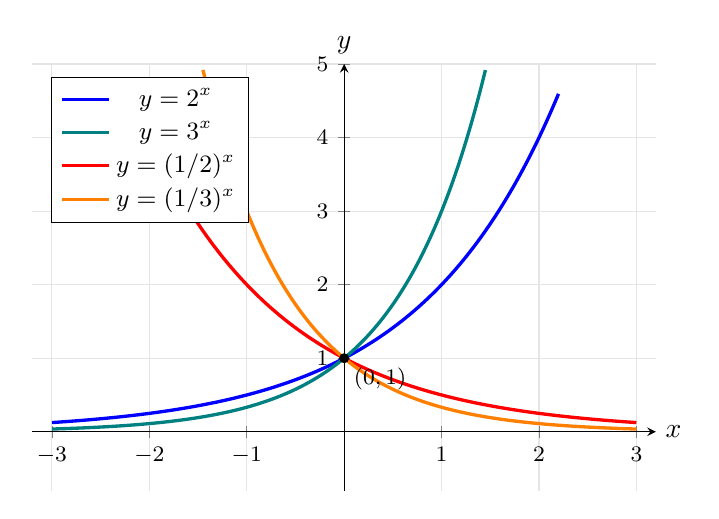
\begin{tikzpicture}
\begin{axis}[
    axis lines=middle,
    xmin=-3.2, xmax=3.2,
    ymin=-0.8, ymax=5.0,
    width=9.5cm, height=7cm,
    xlabel={$x$}, ylabel={$y$},
    xlabel style={right}, ylabel style={above},
    samples=200,
    grid=both,
    grid style={gray!20},
    legend pos=north west,
    legend style={font=\small},
    tick label style={font=\footnotesize},
]
\addplot[blue, very thick, domain=-3:2.2] {2^x};
\addlegendentry{$y=2^x$}
\addplot[teal, very thick, domain=-3:1.45] {3^x};
\addlegendentry{$y=3^x$}
\addplot[red, very thick, domain=-2.2:3] {(1/2)^x};
\addlegendentry{$y=(1/2)^x$}
\addplot[orange, very thick, domain=-1.45:3] {(1/3)^x};
\addlegendentry{$y=(1/3)^x$}
\addplot[only marks, mark=*, mark size=1.6pt, black] coordinates {(0,1)};
\node[below right, font=\footnotesize] at (axis cs:0,1) {$(0,1)$};
\end{axis}
\end{tikzpicture}
\end{document}
